\subsubsection*{Resultados obtenidos}
%Nota: Al ser los resultados de los experimentos sobre ambos tests muy similares, decidimos analizarlos en conjunto.

\subsubsection*{Tests KNN}

Uno de los aspectos más importantes nuestra experimentación es determinar la cantidad óptima de vecínos cercanos, por eso es que vamos a testear el tamaño de K con KNN sin PCA para evitar tener más variables que puedan interferír en nuestra experimencación.




\begin{figure}[H]
\begin{subfigure}[h]{0.62\linewidth}
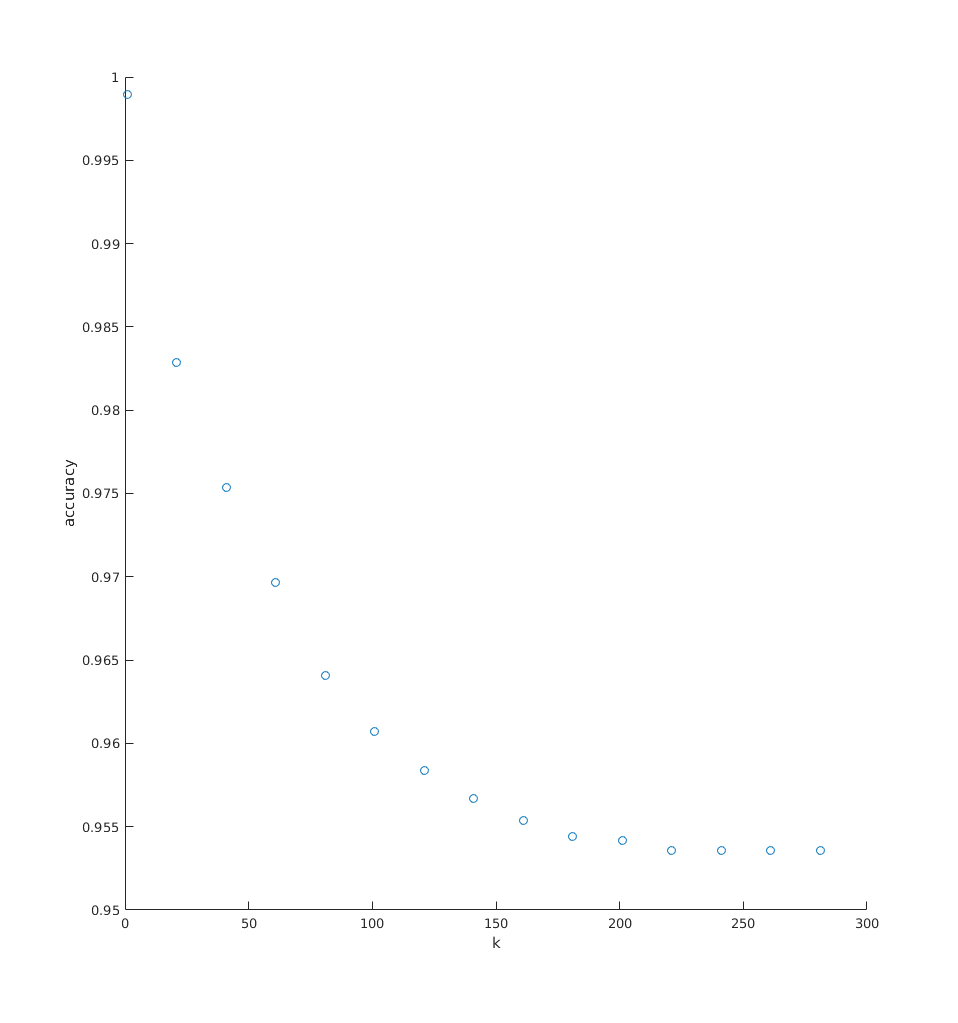
\includegraphics[width=\linewidth]{img/k_knn_accu.png}
\caption{Utilizando imágenes reducidas}
\end{subfigure}
\hfill
\begin{subfigure}[h]{0.62\linewidth}
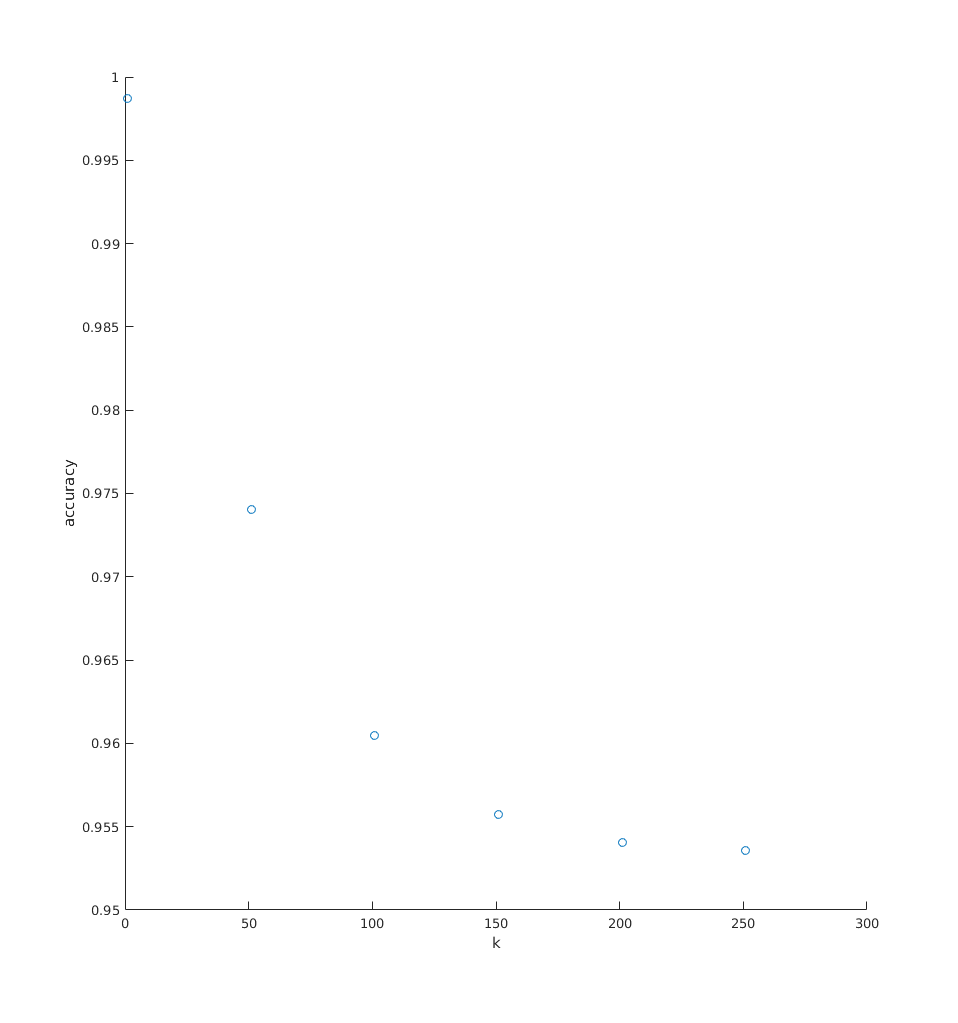
\includegraphics[width=\linewidth]{img/big_k_knn_accu.png}
\caption{Utilizando imágenes grandes}
\end{subfigure}%
\caption{K vs Accuracy con KNN sin PCA}
\end{figure}

%Dados los resultados, en este caso consideramos que utilizando un valor de K cercano a 10 obtenemos la mejor relación (dentro de nuestro set de tests).\newline
%Por un lado evitamos el problema que ocurre cuando K es demasiado grande y por otro, tomamos una cantidad de imágenes cercanas suficiente como para minimizar el impacto de algún outsider. Aun que cabe destacar que en este caso particular K = 1 tuvo un mejor comportamiento de lo que esperabamos, consideramos que sería arriesgado tomarlo como valor confiable con otros sets de imágenes.

%%%%%%%%%%%%%%%%%%%%%%%%%%%%%%%%%%%%%%%%%%%%%%%%%%%%%%%%%%%%%%%%%%%%%
\begin{figure}[H]
	\centering	
	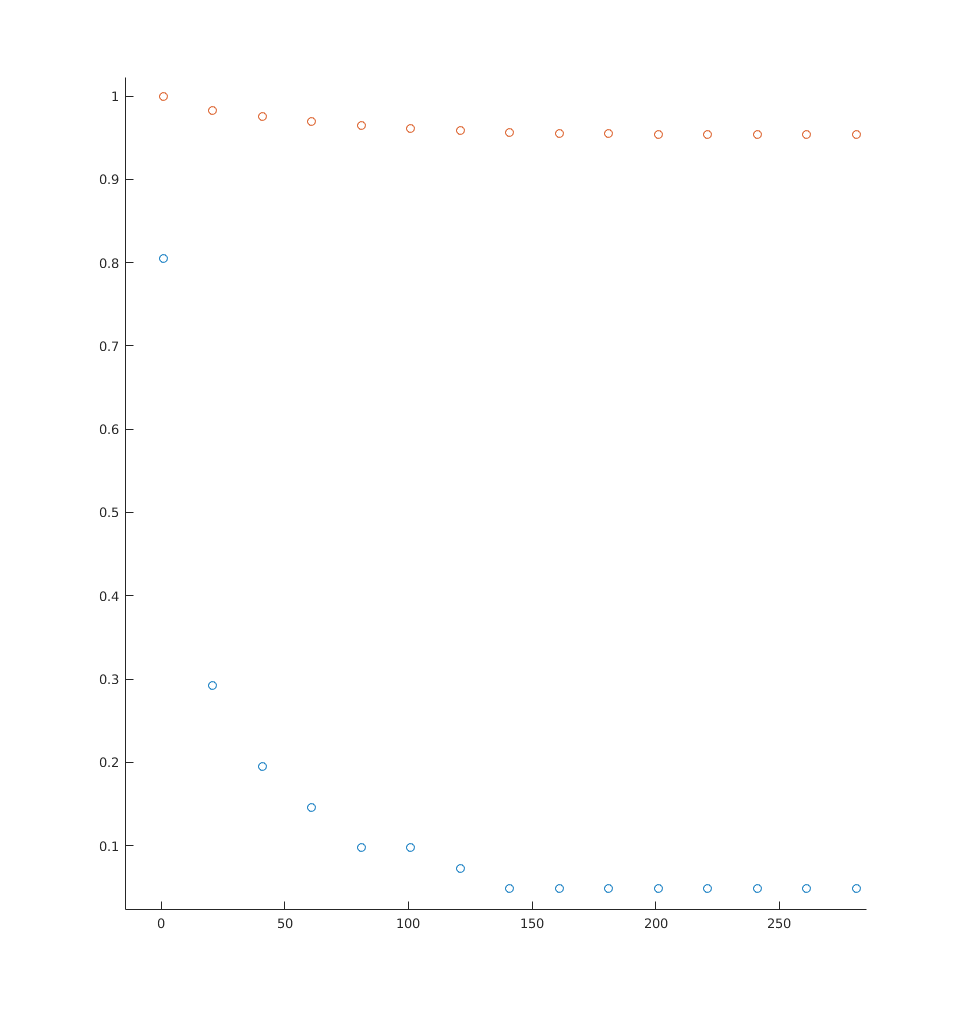
\includegraphics[width=0.8\textwidth]{img/acu_pre.png}
	\caption{Accuracy y precision vs K}
	\label{fig: Accuracy y precision vs K con KNN}
\end{figure}

En este experimento estudiamos la forma en la que la cantidad de vecinos cercanos afecta a las métricas Accuracy y Precisión. Para esto utilizamos el método KNN (sin PCA) para no involucrar más variables dentro del experimento de las necesarias.

Lo que encontramos no fue muy distinto de lo esperado. Antes ya vimos la forma en la que Accuracy variaba en función de la cantidad de vecinos cercanos (Figura 1). Pero como explicamos en cuanto al funcionamiento y elección de un K apropiado para el KNN, un K = 250 por ejemplo no es una buena elección, así que en este caso el accuracy resulta ser una métrica un tanto engañosa.

Para tener un sistema preciso -valga la redundancia- necesitamos un valos de precision relativamente alto. Entonces en función de lo que nos indica el gráfico nuevamente un valor aproximado de K = 1 nos parece una buena opción.
%%%%%%%%%%%%%%%%%%%%%%%%%%%%%%%%%%%%%%%%%%%%%%%%%%%%%%%%%%%%%%%%%%%%%
\begin{figure}[H]
\begin{subfigure}[h]{0.62\linewidth}
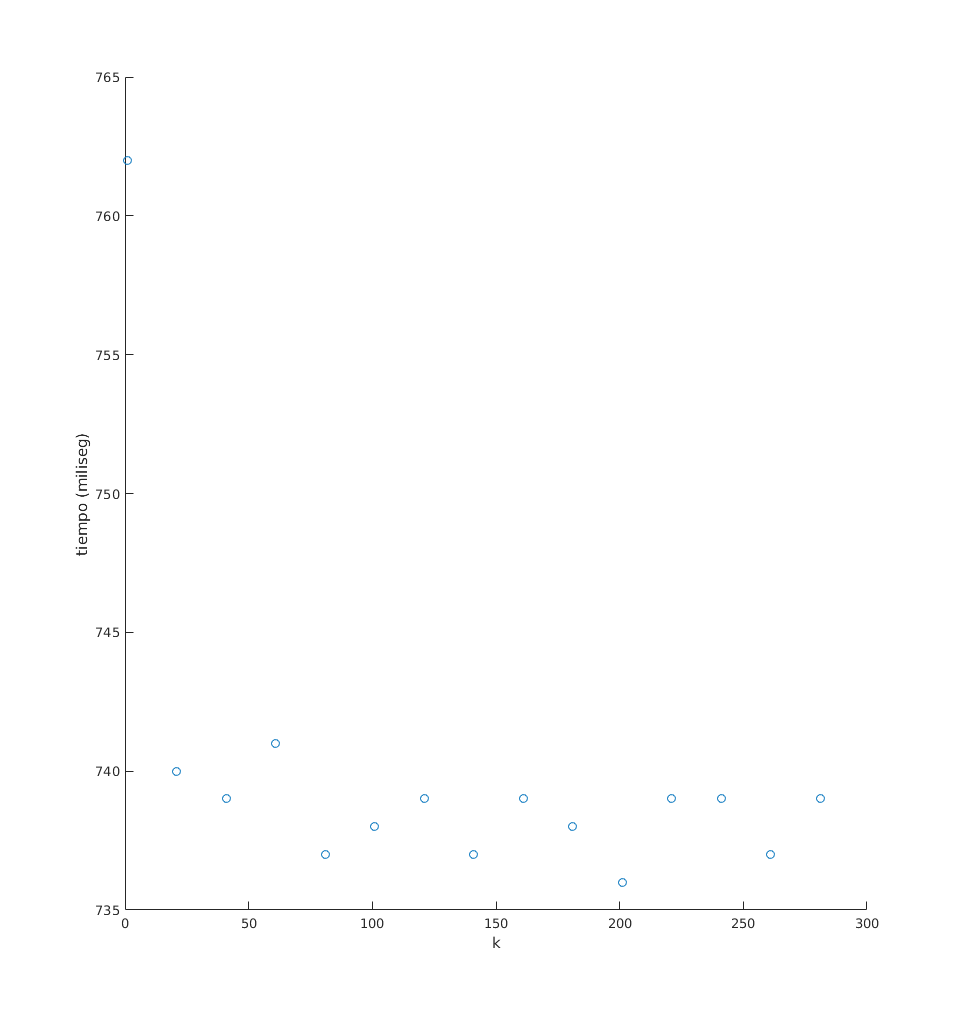
\includegraphics[width=\linewidth]{img/k_knn_tiempo.png}
\caption{Utilizando imágenes reducidas}
\end{subfigure}
\hfill
\begin{subfigure}[h]{0.62\linewidth}
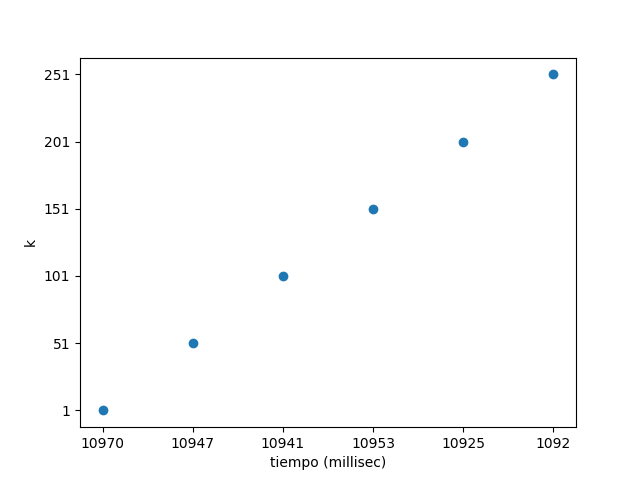
\includegraphics[width=\linewidth]{img/big_k_knn_tiempo.png}
\caption{Utilizando imágenes grandes}
\end{subfigure}%
\caption{K vs tiempo con KNN sin PCA}
\end{figure}


En estos tests obtuvimos resultados coherentes con lo esperado.
Lo único que podemos señalar es un tiempo mayor en PCA a lo que uno podría intuir, pero esto se debe a la aplicación de PCA en cada ejecución. En un uso real esperaríamos encontrar una reducción del tiempo de ejecución de KNN+PCA en relación al KNN.

%%%%%%%%%%%%%%%%%%%%%%%%%%%%%%%%%%%%%%%%%%%%%%%%%%%%%%%%%%%%%%%%%%%%%



\subsubsection*{Conclusiones del test}
Dados los resultados resulta evidente que cuánto más chico el K mejor se comportan nuestras métricas, luego concluímos que K = 1 es el valor óptimo.
Esto tiene sentido, sin embargo si tuvieramos que implementar este problema en la vida real creemos que nos encontraríamos con outlayers que pueden afectar el resultado, ya que con un solo vecino cercano tenemos un sistema poco robusto.






%%%%%%%%%%%%%%%%%%%%%%%%%%%%%%%%%%%%%%%%%%%%%%%%%%%%%%%%%%%%%%%%%%%%%
\subsubsection*{Test con KNN + PCA}
Ahora vamos a evaluar como se comporta nuestra implementación con PCA, para eso vamos a repetir los tests anteriores pero esta vez utilizando KNN + PCA.
De acuerdo a lo concluído de los tests anteriores inferimos que utilizar K = 1 o algún valor cercano sería lo mejor. 



%%%%%%%%%%%%%%%%%%%%%%%%%%%%%%%%%%%%%%%%%%%%%%%%%%%%%%%%%%%%%%%%%%%%%
\begin{figure}[H]
	\centering
	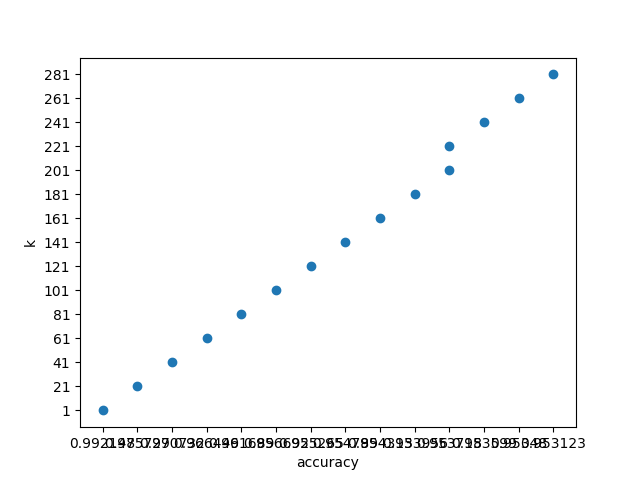
\includegraphics[width=0.8\textwidth]{img/k_pca_accu.png}
	\caption{Accuracy vs K con KNN + PCA}
	\label{fig:K vs Accuracy con KNN + PCA}
\end{figure}

En este caso vemos una estrecha relación entre cuantos vecinos cercanos tomamos y el accuracy.
Esto se debe a que al tomar más vecinos cercanos nos exponemos a un error mayor debido a que le estaríamos dando el mismo peso a todos esos K vecinos sin importar que tan cerca estén de la imagen testeada.
Llevando esto a un extremo podríamos tomar $K$ = “Tamano de matriz de entrenamiento”  cualquiera de las clases tendría el mismo peso con lo que perdería sentido este método.
Por otro lado tampoco es conveniente tener un $K$ demasiado chico. Por ejemplo, si tomaramos $K = 1$ asociaríamos la imagen a testear con la que esté a menor distancia, que debido a alguna diferencia la forma en que fue tomada la imagen puede no pertenecer a la clase de la imagen testeada.


%%%%%%%%%%%%%%%%%%%%%%%%%%%%%%%%%%%%%%%%%%%%%%%%%%%%%%%%%%%%%%%%%%%%%

\begin{figure}[H]
\begin{subfigure}[h]{0.62\linewidth}
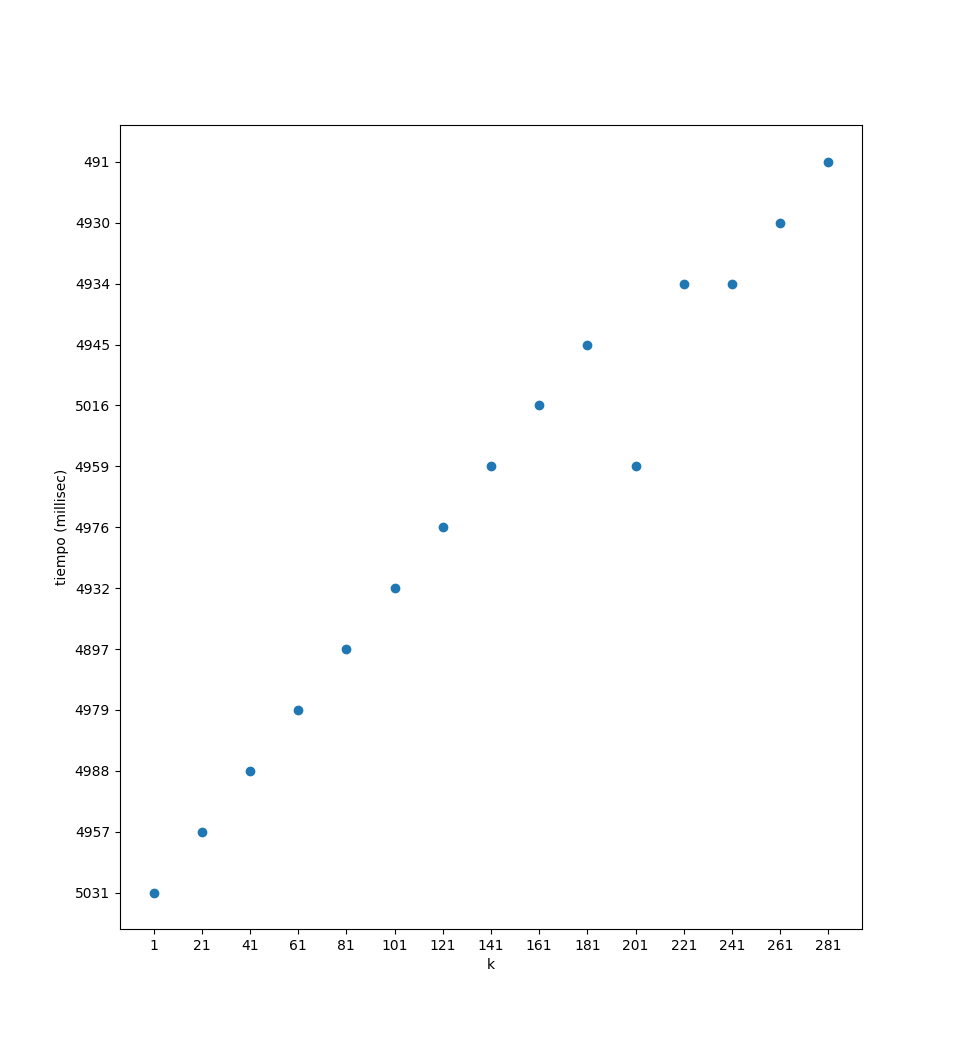
\includegraphics[width=\linewidth]{img/k_pca_tiempo.png}
\caption{Utilizando imágenes reducidas}
\end{subfigure}
\hfill
\begin{subfigure}[h]{0.62\linewidth}
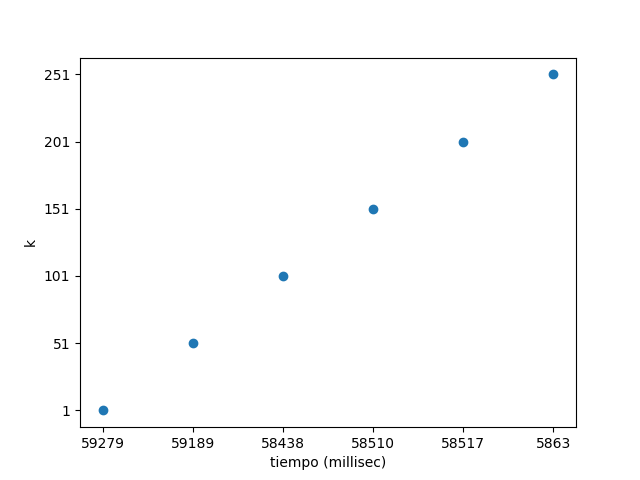
\includegraphics[width=\linewidth]{img/big_k_pca_tiempo.png}
\caption{Utilizando imágenes grandes}
\end{subfigure}%
\caption{K vs tiempo con KNN+PCA}
\end{figure}



%%%%%%%%%%%%%%%%%%%%%%%%%%%%%%%%%%%%%%%%%%%%%%%%%%%%%%%%%%%%%%%%%%%%%



\begin{figure}[H]
\begin{subfigure}[h]{0.62\linewidth}
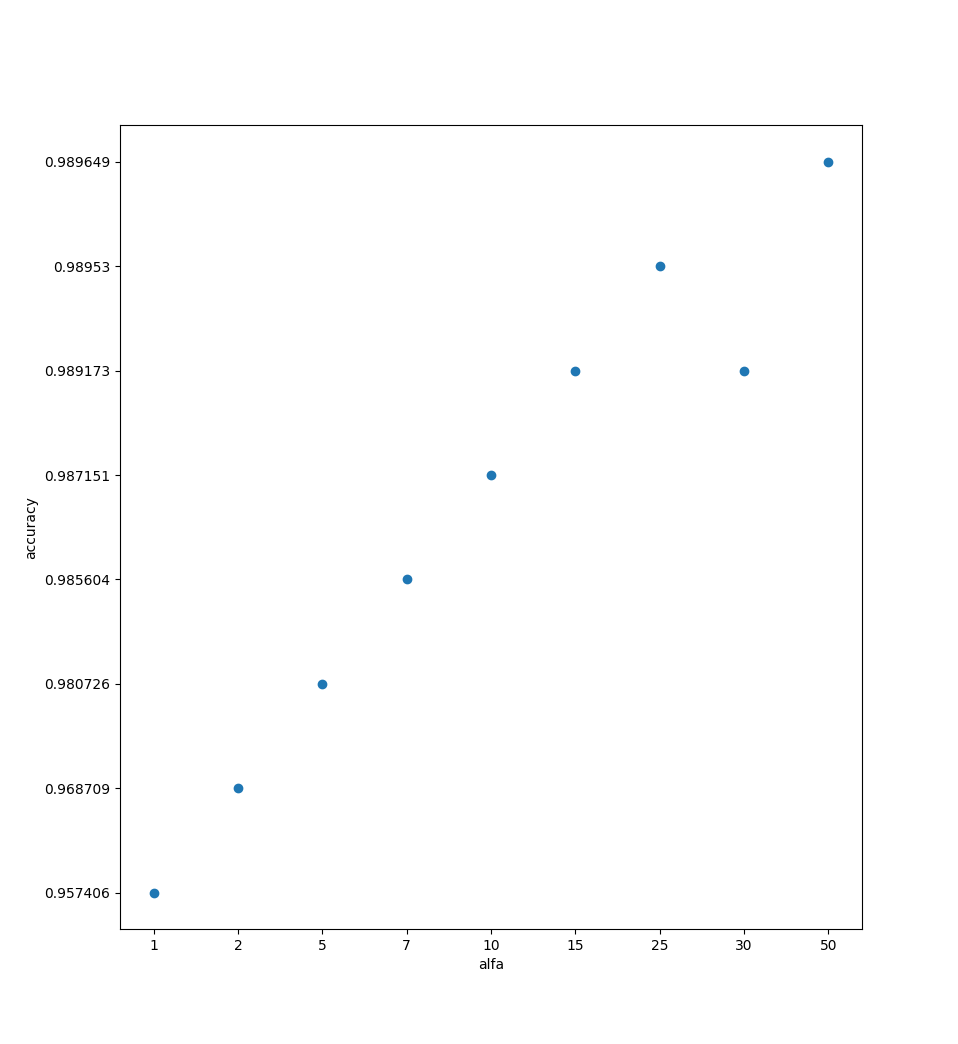
\includegraphics[width=\linewidth]{img/alfa_pca_accu.png}
\caption{Utilizando imágenes reducidas}
\end{subfigure}
\hfill
\begin{subfigure}[h]{0.62\linewidth}
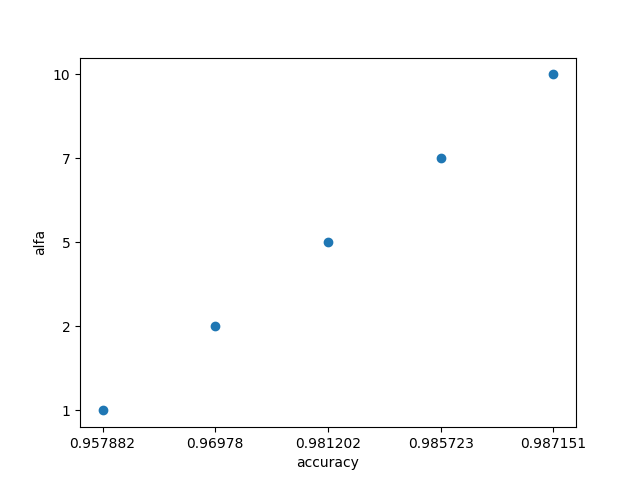
\includegraphics[width=\linewidth]{img/big_alfa_pca_accu.png}
\caption{Utilizando imágenes grandes}
\end{subfigure}%
\caption{Accuracy vs $\alpha$ con KNN+PCA}
\end{figure}

En este caso podemos observar una relación entre las dos variables, a medida que el $\alpha$ aumenta vemos como también lo hace nuestro accuracy.
Como expresamos anteriormente, debido al funcionamiento de PCA esperábamos que a mayor $\alpha$, mejores sean nuestros resultados (todas nuestras métricas en general) y por lo tanto nuestro accuracy también.

Pero a su vez tambien vimos que un $\alpha$ muy elevado  nos elevaría el tiempo de ejecución y a su vez en este gráfico vemos como las diferencias entre accuracy son cada vez menores (por ejemplo entre $\alpha$ = 10 y $\alpha$ = 50).

En base a los resultados obtenidos concluimos que un valor de $\alpha$ cercano a 10 nos daría un buen balance entre relativamente la cantidad de componentes principales y la efectividad (se sacrifica algo de efectividad pero a cambio trabajamos con imágenes mucho más chicas, reduciendo el tiempo de ejecución).

%%%%%%%%%%%%%%%%%%%%%%%%%%%%%%%%%%%%%%%%%%%%%%%%%%%%%%%%%%%%%%%%%%%%%
\begin{figure}[H]
\begin{subfigure}[h]{0.62\linewidth}
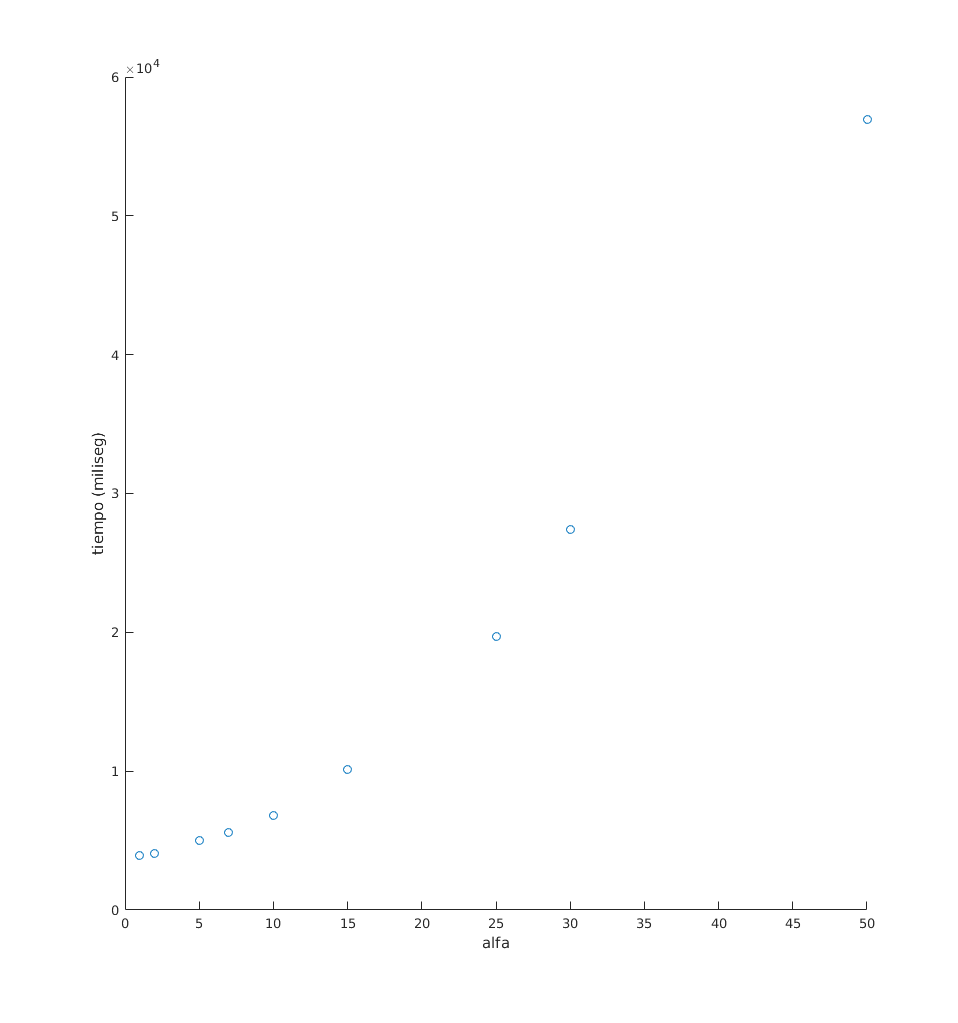
\includegraphics[width=\linewidth]{img/alfa_pca_tiempo.png}
\caption{Utilizando imágenes reducidas}
\end{subfigure}
\hfill
\begin{subfigure}[h]{0.62\linewidth}
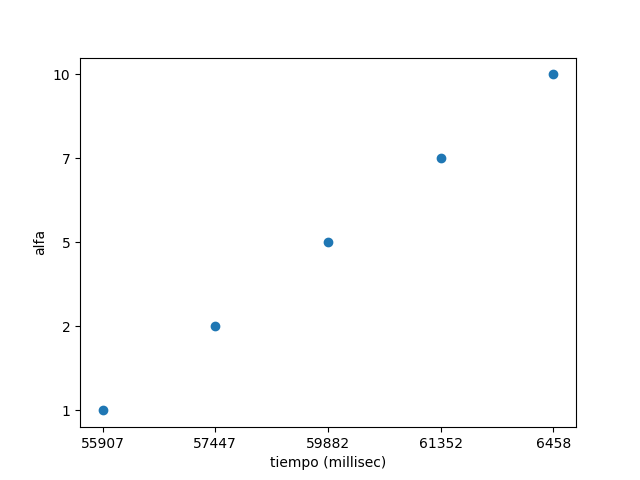
\includegraphics[width=\linewidth]{img/big_alfa_pca_tiempo.png}
\caption{Utilizando imágenes grandes}
\end{subfigure}%
\caption{Tiempo vs $\alpha$ con KNN+PCA}
\end{figure}

Tal como esperabamos vemos que a medida que el $\alpha$ aumenta (es decir, cuantas más componentes principales tengamos), el tiempo de ejecución también lo hace.

Luego, en línea con los resultados de los gráficos anteriores (Accuracy vs $\alpha$) podemos volver a afirmar que un $\alpha$ cercano a 10 sería un buen balance. En este gráfico notamos si tomaramos $\alpha$ = 30, tardaría aproximadamente el triple y no obtendríamos una mejora sustancial en el accuracy.
%%%%%%%%%%%%%%%%%%%%%%%%%%%%%%%%%%%%%%%%%%%%%%%%%%%%%%%%%%%%%%%%%%%%%



Es llegamos a la conclusión de que utilizando un valor de K cercano a 10 obtenemos la mejor relación (dentro de nuestro set de tests).
Por un lado evitamos el problema que ocurre cuando K es demasiado grande y por otro, tomamos una cantidad de imágenes cercanas suficiente como para minimizar el impacto de algún outsider.


